%\documentclass[11pt,a4paper]{scrartcl}
\documentclass{MSM_latex}
\author{M. Denkinger, S. Eyes, J. Schnitzler}


\makeatletter
\let\runauthor\@author
\let\rundate\@date
% Fußzeile
\lfoot{\textit{\runauthor} \\ \textit{\rundate}}




\begin{document}
\section{Weihnachtsprojekt: Simulation und Regelung eines Knickarmroboters}

\subsection*{Aufgabe 1 - Bestimmung der Kinematik und DH-Parameter}

Zur Bestimmung der Kinematik ist es notwendig herauszufinden, wie die einzelnen Gelenke des Roboters miteinander verbunden sind.
Die Denavit-Hartenberg-Notation wird verwendet, um die 3D-Transformation zum nächsten Gelenk mithilfe von vier Parameter zu beschreiben. Im Fall des Knickarmroboters ist
dies sehr einfach, da es sich lediglich um eine Kette von drei Gelenken handelt. Die Koordinatentransformation ist jeweils eine Rotation um die $z$-Achse mit $\theta_i$
und eine Translation in der $xy$-Ebene, um die Länge $a_i = l_i$. Wir können somit das erste Gelenk in den Ursprung legen und mithilfe von zwei Transformationen $T_{12}$ und $T_{23}$ alles beschreiben. Um mit einem nicht gedrehten Koordinatensystem anzufangen, benötigen wir zusätzlich $T_{01}$. Die DH-Parameter sind in Tabelle \ref{tab:DH} aufgeführt.



\begin{table}[tb]
	\centering
	\begin{tabular}{lccccr}
		\toprule
		Achse & $a_{i-1}$ & $\alpha_{i-1}$ & $d_i$ & $\theta_i$ & Art \\
		\midrule
		1 & 0& 0& 0& $-90^\circ $& Rotation \\
		2 & $l_1 = 0.16 \text{ m}$& 0& 0& $\alpha$& Translation\\
		3 & $l_2 = 0.128 \text{ m}$& 0& 0& $\beta$& Both\\ 
		\bottomrule
	\end{tabular}
	\caption{DH-Parameter des Knickarmroboters}
	\label{tab:DH}
\end{table}

Daraus resultieren die Transformationsmatrizen
\begin{equation*}
	T_{12}(\alpha, l_1) = \begin{pmatrix}
	\cos(\alpha) & -\sin(\alpha) & 0 & 0 \\
	\sin(\alpha) & \cos(\alpha) & 0 & 0 \\
	0 & 0 & 1 & 0 \\
	0 & 0 & 0 & 1
	\end{pmatrix} \cdot \begin{pmatrix}
	1 & 0 & 0 & l_1 \\
	0 & 1 & 0 & 0 \\
	0 & 0 & 1 & 0 \\
	0 & 0 & 0 & 1
	\end{pmatrix} = \begin{pmatrix}
	\cos(\alpha) & -\sin(\alpha) & 0 & \cos(\alpha) l_1 \\
	\sin(\alpha) & \cos(\alpha) & 0 & \sin(\alpha) l_1 \\
	0 & 0 & 1 & 0 \\
	0 & 0 & 0 & 1
	\end{pmatrix}
\end{equation*}
und
\begin{equation*}
	T_{23}(\beta, l_2) = \begin{pmatrix}
	\cos(\beta) & -\sin(\beta) & 0 & 0 \\
	\sin(\beta) & \cos(\beta) & 0 & 0 \\
	0 & 0 & 1 & 0 \\
	0 & 0 & 0 & 1
	\end{pmatrix} \cdot \begin{pmatrix}
	1 & 0 & 0 & l_2 \\
	0 & 1 & 0 & 0 \\
	0 & 0 & 1 & 0 \\
	0 & 0 & 0 & 1
	\end{pmatrix} = \begin{pmatrix}
	\cos(\beta) & -\sin(\beta) & 0 & \cos(\beta) l_2 \\
	\sin(\beta) & \cos(\beta) & 0 & \sin(\beta) l_2 \\
	0 & 0 & 1 & 0 \\
	0 & 0 & 0 & 1
	\end{pmatrix}
\end{equation*}

Die Gesamttransformation ergibt sich aus der Multiplikation der beiden Matrizen, welche mithilfe von trigonometrischen Additionstheoremen vereinfacht werden kann.

\begin{equation*}
	T_{13} = T_{12} \cdot T_{23} = \begin{pmatrix}
	\cos(\alpha + \beta) & -\sin(\alpha + \beta) & 0 & \cos(\alpha) l_1 + \cos(\alpha + \beta) l_2\\
	\sin(\alpha + \beta) & \cos(\alpha + \beta) & 0 & \sin(\alpha) l_1 + \sin(\alpha + \beta) l_2 \\
	0 & 0 & 1 & 0 \\
	0 & 0 & 0 & 1
	\end{pmatrix}
\end{equation*}

\begin{equation*}
	T_{03} = \begin{pmatrix}
	\cos(\alpha + \beta) & -\sin(\alpha + \beta) & 0 & \cos(\alpha) l_1 + \cos(\alpha + \beta) l_2\\
	\sin(\alpha + \beta) & \cos(\alpha + \beta) & 0 & \sin(\alpha) l_1 + \sin(\alpha + \beta) l_2 \\
	0 & 0 & 1 & 0 \\
	0 & 0 & 0 & 1
	\end{pmatrix}
\end{equation*}

Somit ergibt sich die Position von Gelenk 2 im Weltkoordinatensystem zu
\begin{equation*}
	\begin{pmatrix} x_2 \\ y_2 \\ z_2 \end{pmatrix} = \begin{pmatrix}
	\cos(\alpha) l_1\\ \sin(\alpha) l_1 \\ z_2 \end{pmatrix}
\end{equation*}
und die Position von Gelenk 3 bzw. des Endeffektors zu
\begin{equation*}
	\begin{pmatrix} x_3 \\ y_3 \\ z_3 \end{pmatrix} = 
	\begin{pmatrix}
	\cos(\alpha) l_1 + \cos(\alpha + \beta) l_2\\ \sin(\alpha) l_1 + \sin(\alpha + \beta) l_2 \\ z_3 
	\end{pmatrix}
\end{equation*}

\textit{Anmerkung}: Da die Parameter $\alpha_{i-1}$ und $d_i$ sind immer null sind, ist eine 2D Betrachtung ausreichend, wie man auch an der \emph{Identitäts-Zeile-Spalte} für $z$ erkennen kann.

\subsection*{Aufgabe 2 - Bestimmung der Bewegungsgleichung}

\subsubsection*{Generalisierte Koordinaten}
Die Wahl fällt zu $q_1 = \alpha$ und $q_2 = \beta$. Die generalisierten Koordinaten sind somit die Winkel der Gelenke 2 und 3.

\subsubsection*{Lagrang'sche Gleichungen}

\paragraph*{Jacobi-Matrizen}



\paragraph*{potentielle Energie $U$}



\newpage


\section*{Template}


% following notes can be excluded for the actual documentation
\textit{Guidelines:} Die Ergebnisse des Weihnachtsprojekts sollten mit Hilfe der vorgegebenen Vorlage  visualisiert und diskutiert werden. 
Der Bericht sollte dabei eine maximale Länge von acht Seiten nicht überschreiten, die Aufgabenstellung wird hierbei nicht erneut aufgeführt. 
Zur Darstellung und Diskussion können die angehängten Tabellen- und Abbildungsvorlagen verwendet werden, siehe Tab.~\ref{tab:DH} sowie Abb.~\ref{fig:Roboter} und~\ref{fig:plot_example}. 
Etwaige Literatur sollte sauber referenziert werden, z.B. mittels Bibtex~\cite{FehrSchmidSchneiderEberhard20,Fuchs23, DenavitHartenberg55,Lipkin05}.

\textit{Software Guidelines:}
Zusätzlich zur Dokumentation sollen die Simulationsdateien abgegeben werden.
Es ist auf eine ausreichende Kommentierung der Skripte und Funktionen zu achten, numerische Parameter sollen mittels eines Initialisierungsskripts eingebunden werden.

\textit{Gruppenarbeit:}
Es bietet sich an Simulations- und Dokumentationsdateien mit Hilfe von Versionskontrolle gemeinsam zu verwalten, beispielsweise durch den Github-Server der Universität Stuttgart, siehe \href{https://www.tik.uni-stuttgart.de/dienste-a-z/Git-Hosting/}{TIK GitHub}.

% actual documentation starting ...
%\setcounter{section}{0}
%\section{Modifizierte DH-Parameter und Vorwärtskinematik}



\clearpage
%\subsection*{Vorlagen}


\begin{figure}[t]
	\centering
	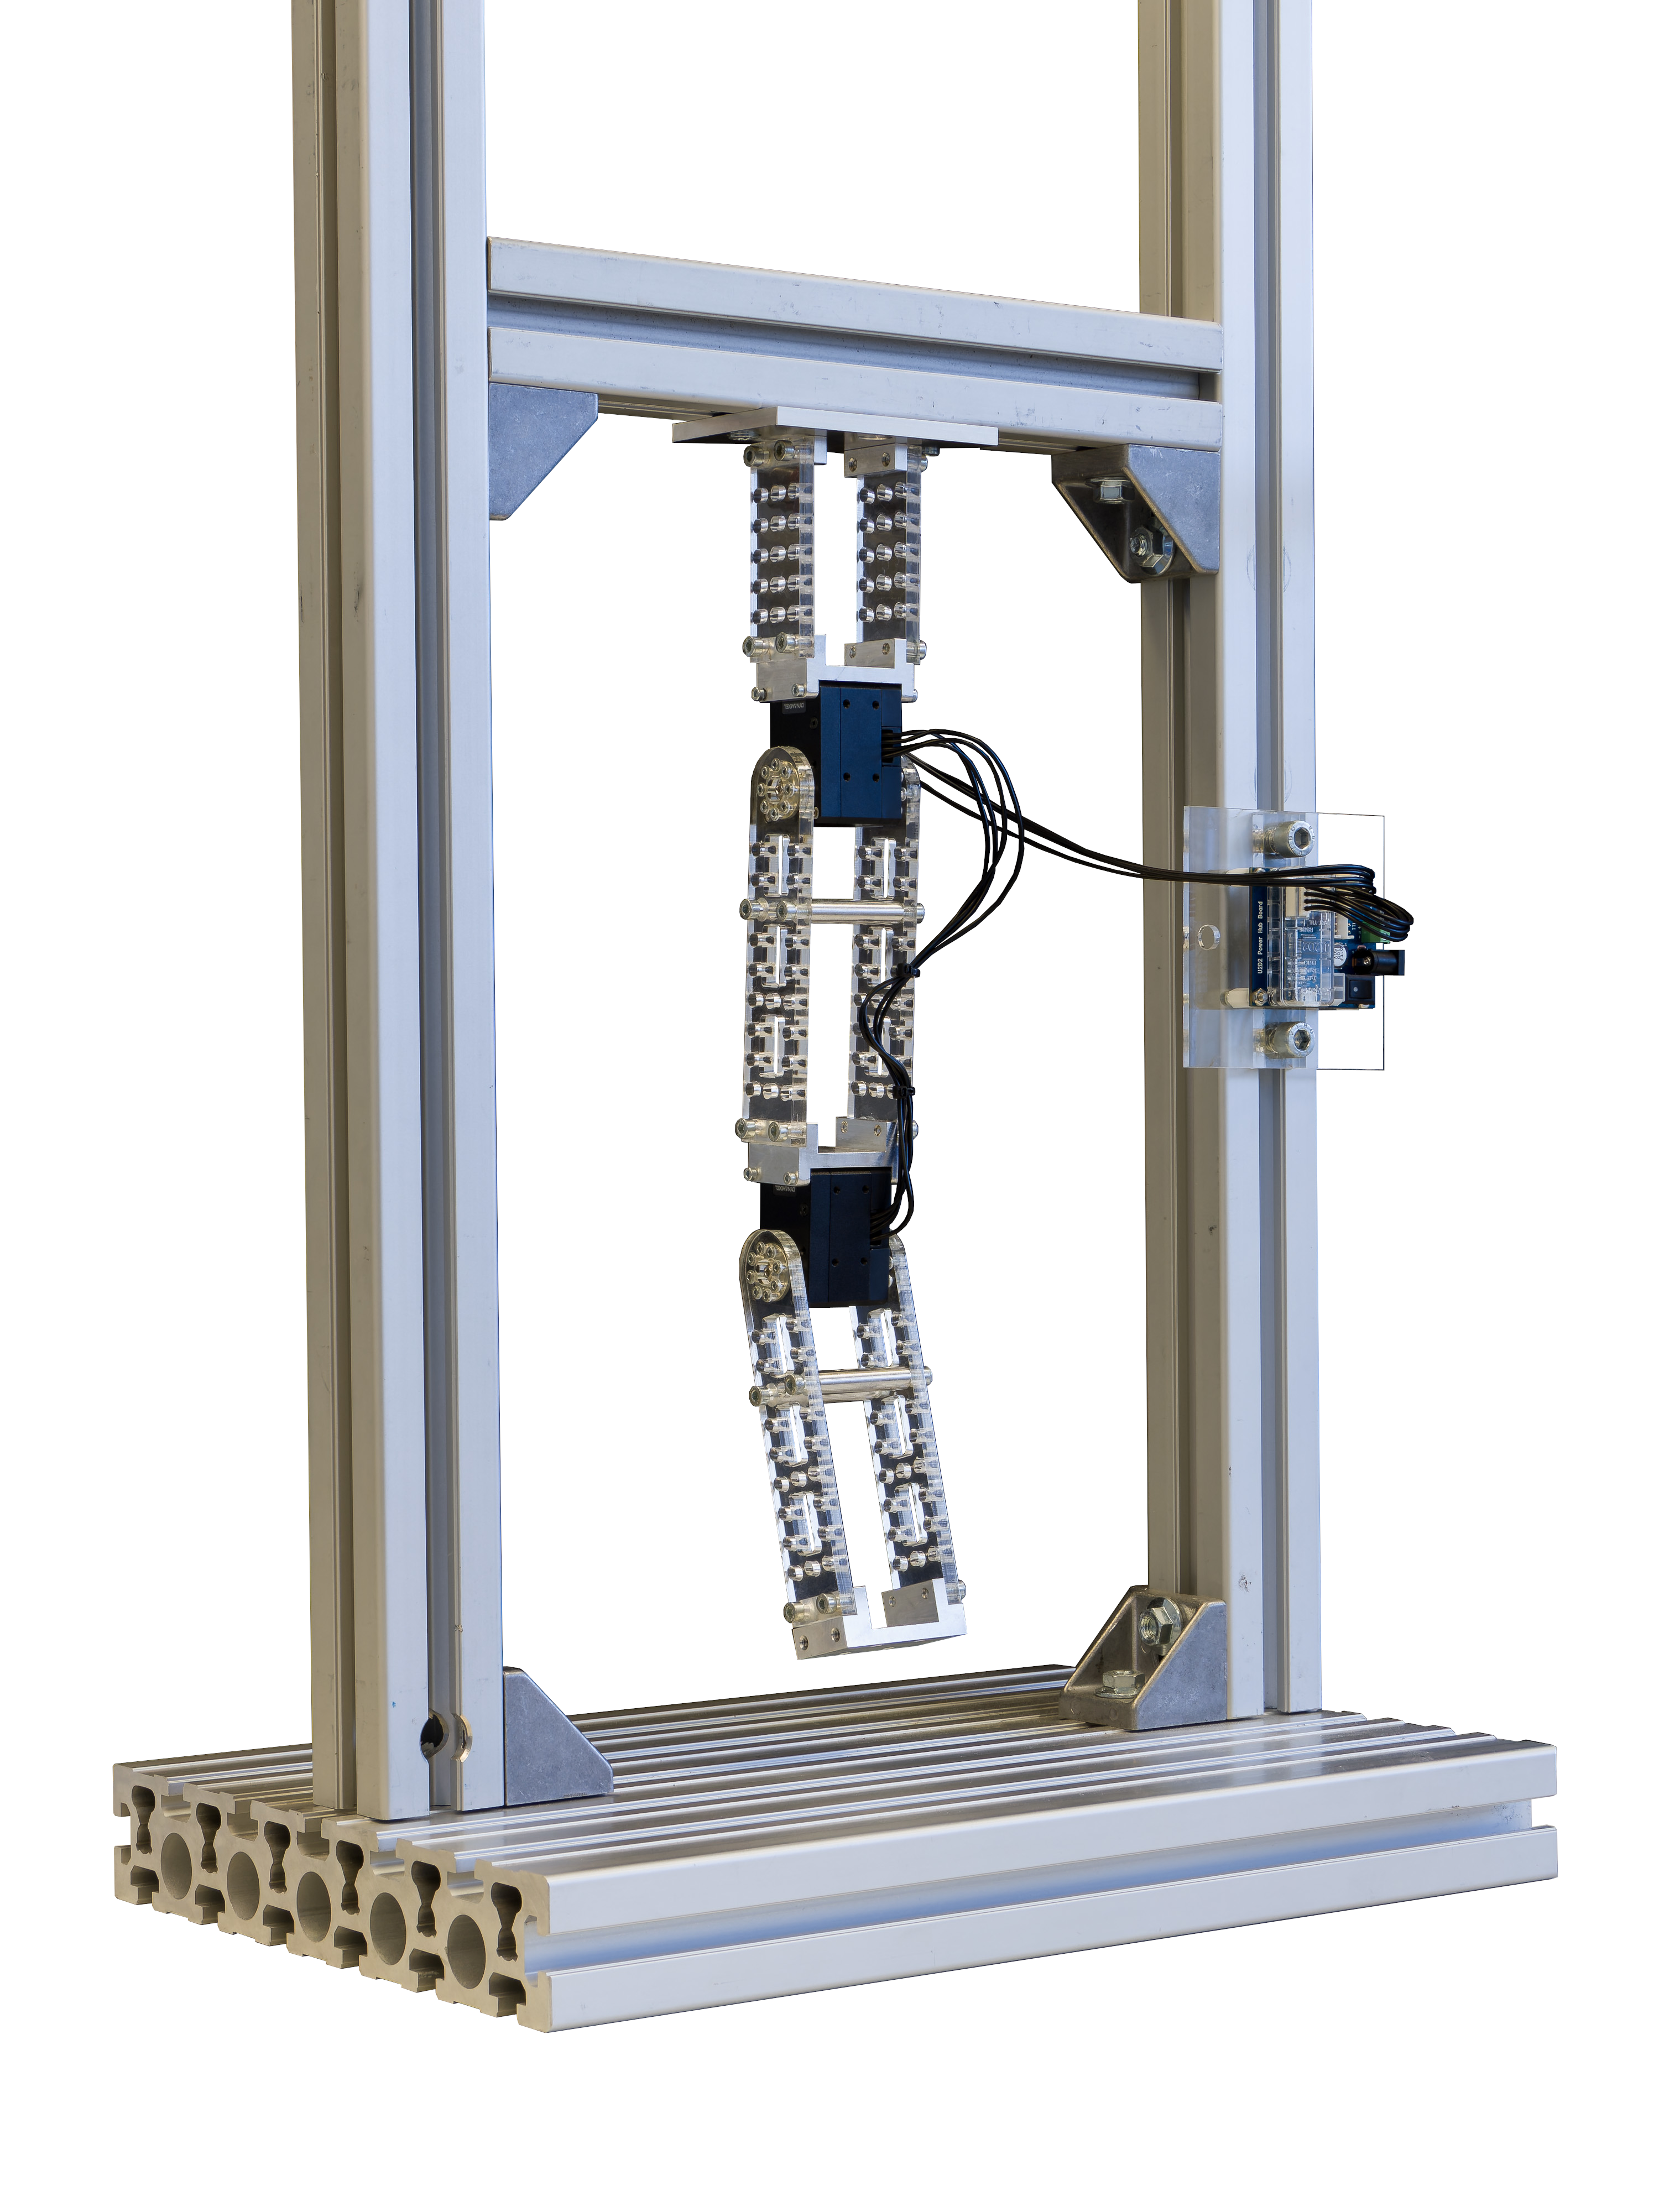
\includegraphics[height=7cm]{img/Versuchsaufbau.png}
	%	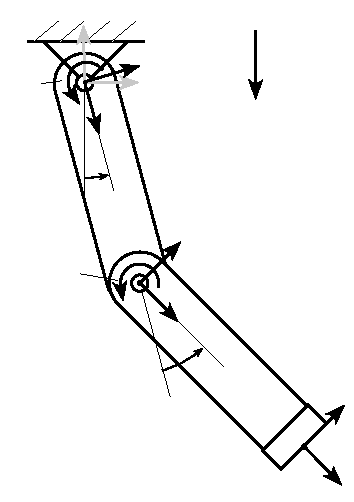
\includegraphics[height=7cm]{img/Zeichnung/Zeichnung.pdf}
	\hspace{1cm}
	\def\svgwidth{5.5cm}
	\input{img/Zeichnung/Zeichnung.pdf_tex}
	\caption{Foto sowie schematische Darstellung des zu untersuchenden Roboters~\cite{Fuchs23}.}
	\label{fig:Roboter}
\end{figure}

\def\myLineWidth{1.5pt}

% may define colors in advance, e.g., if they should be the same throughout the article
\definecolor{mycolor1}{cmyk}{100,70,0,0}%
\definecolor{mycolor2}{RGB}{255, 68, 76}% 
\begin{figure}[t]
	\centering
	% Minimal example for a TikZ plot

% 1) begin the overall picture
\begin{tikzpicture} 
    % 2) begin the axis
    \begin{axis}[%
        % 2a) define the properties of the axis
        width=\textwidth,   % width of the plot
        height= 5cm,       % height of the plot
        xmajorgrids,        % grid on
        xmin = -1,
        xmax = 11,
        ymajorgrids,
        ylabel={Auslenkung $\unit[y]{(m)}$},  % axis label (unit needs units-package)
        xlabel={Zeit $\unit[t]{(s)}$}
        ]
        
        % further may necessary setting:
%        xtick={0.5*pi, pi, 1.5*pi, 2*pi},   % modified xtick positions
%        xticklabels={$\pi/2$,$\pi$,$\nicefrac{3\pi}{2}$,$2\pi$},              % labels at previously set positions
%        ytick={-1,0,1},                 % analogous to x-ticks
%        yticklabels={-$\hat{y}$,0,$\hat{y}$}, 

%        ylabel={displacement $\unit[y]{(m)}$},  % axis label
%        % define legend
%        legend style={
%        	draw=black, % color of the border
%        	at={(0.5,1.05)}, % position plot has normalized wodth and length of 1
%        	anchor = south, % set legend at which anchor to defined position
%        	legend columns = 2, % legend entries in two columns
%        	/tikz/every even column/.append style={column sep=0.5cm} % space between legend's columns
%        }
%        ]
        
        
        % 2b) the plots itselves
        
        % insert data from txt-file
        \addplot[color = mycolor1, line width = \myLineWidth] table{img/plots/data/sin_data.txt}; % define plot properties in [...]
        \addlegendentry{$\sin$} % add legend entry

        \addplot[color = mycolor2, line width = \myLineWidth, dashdotted] table{img/plots/data/cos_data.txt}; % insert data from txt-file
        \addlegendentry{$\cos$} % add legend entry
        
        % manual plot
        \addplot[color = black, line width = 2.0, opacity = 0.5, forget plot] table[row sep=crcr] {%
        	%
        	-5	1\\
        	15 1\\
        }; 
    
    \end{axis}
    
\end{tikzpicture}%

	\caption{Beispielhafter Plot}
	\label{fig:plot_example}
\end{figure}

\bibliographystyle{itm_phd_deu}
\bibliography{literature.bib}

\end{document}